% !TeX root = ../../main.tex
\subsection{Control denominators recover interactions under composition shifts}
\label{sec:simcrispr}

We next used simCRISPR to generate a factorial knockout-by-treatment screen
with a known guide-level interaction \citep{zhu2026simcrispr}.  Each of three
seeds contained 2,000 sgRNAs and three independent replicates per factorial
arm.  Non-targeting guides had a true interaction of zero, and safe-harbor
guides separated the effect of cutting from a targeted gene effect.  Each
control class was split so that normalization and calibration guides were
never used for evaluation.

\begin{table}[ht]
\centering
\caption{Interaction recovery in simCRISPR (three-seed mean).  Recall and F1
use targeting guides with $|\mathrm{interaction}|\geq0.2$ as positives.  Null
and safe-harbor rates are held-out call fractions at FDR 0.10.}
\label{tab:simcrispr}
\small
\setlength{\tabcolsep}{5pt}
\begin{tabular}{llrrrr}
\toprule
Method & Denominator & Dir.\ recall & F1 & Null rate & Safe-harbor\\
\midrule
BARCS-ST & Library &
0.376 & 0.488 & 0.004 & 0.002\\
BARCS-MOD & Library &
0.375 & 0.481 & 0.000 & 0.000\\
\midrule
BARCS-ST & Non-targeting &
0.769 & 0.870 & 0.024 & 0.070\\
BARCS-MOD & Non-targeting &
\textbf{0.838} & \textbf{0.917} & 0.040 & 0.080\\
\midrule
BARCS-ST & Safe-harbor &
0.762 & 0.864 & 0.042 & 0.042\\
BARCS-MOD & Safe-harbor &
0.830 & 0.914 & 0.027 &
\textbf{0.035}\\
\midrule
MAGeCK-MLE & Non-targeting &
0.003 & 0.006 & 0.000 & 0.000\\
\bottomrule
\end{tabular}
\end{table}

The full-library denominator preserved effect ranking but shifted the
true-zero guides because widespread depletion increased every surviving
guide's library share.  BARCS-MOD consequently reached F1 0.481 with the
library denominator, compared with 0.917 and 0.914 using non-targeting and
safe-harbor denominators.  The held-out null rates remained below the nominal
0.10 in all cases.  The result identifies denominator choice, rather than the
interaction coefficient itself, as the source of the power loss.

\begin{figure}[htbp]
\centering
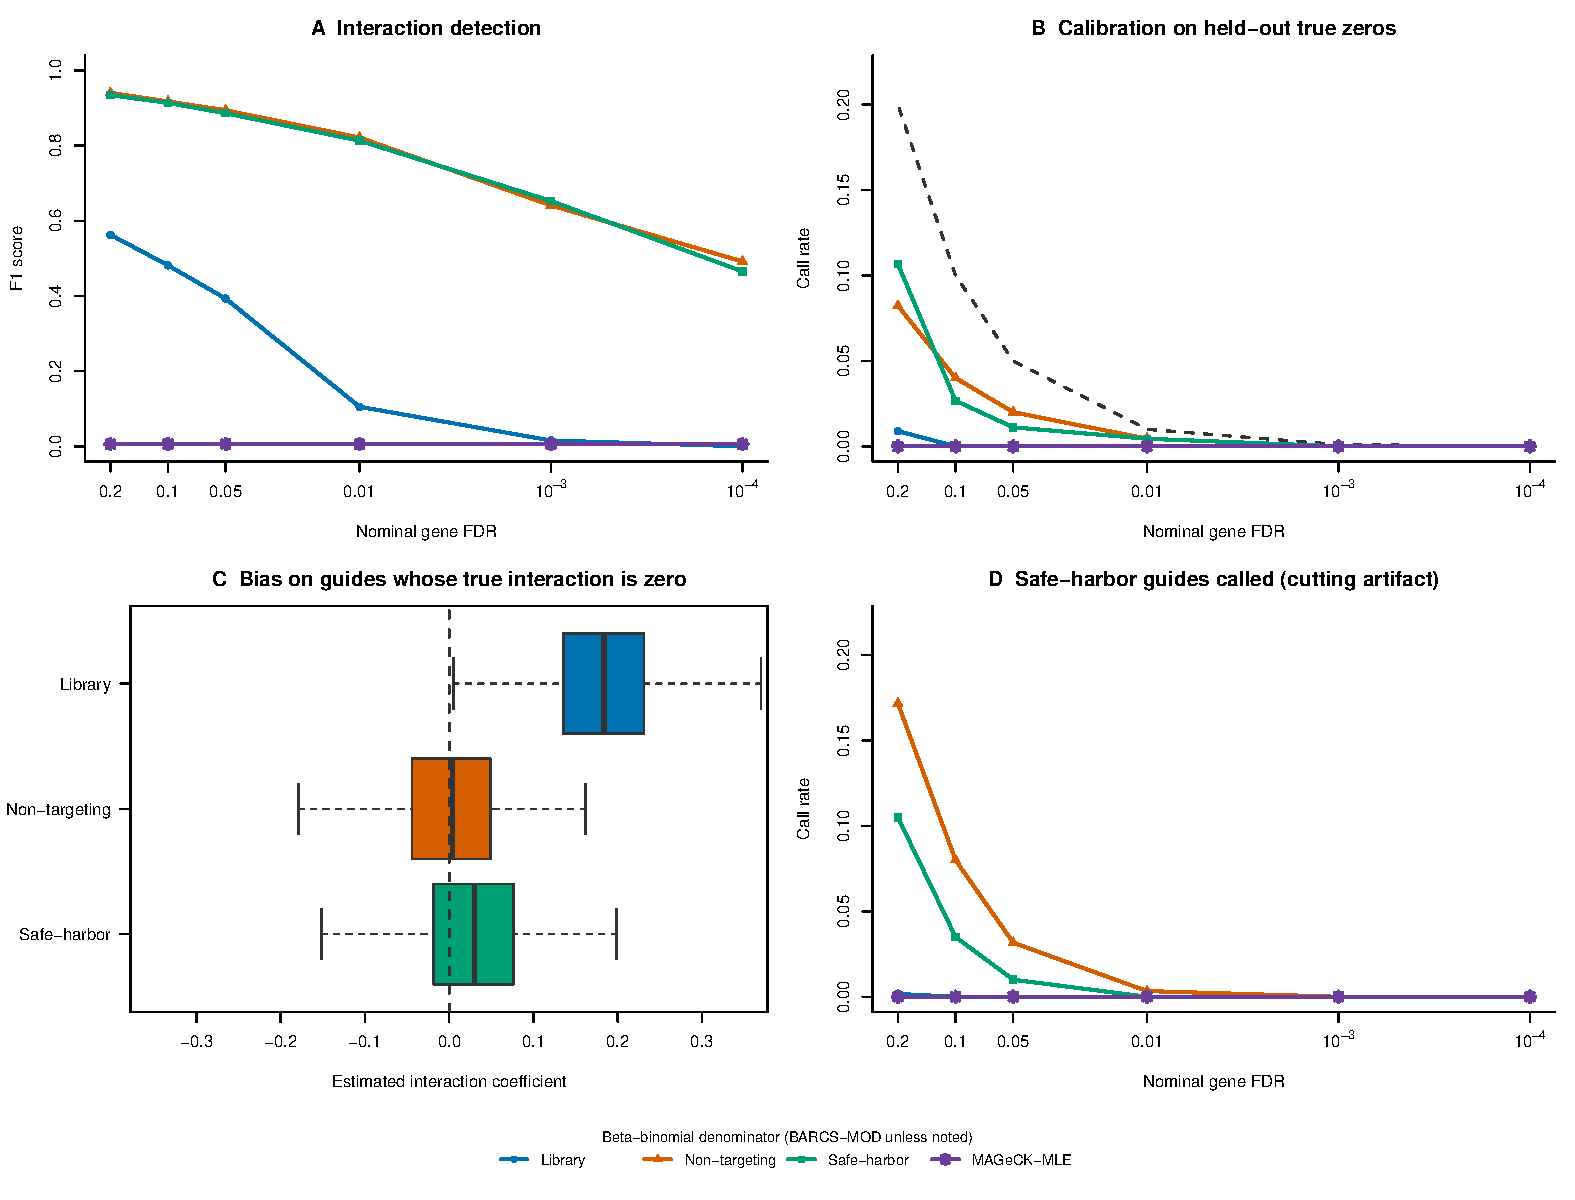
\includegraphics[width=\textwidth]{figures/simcrispr_interaction.pdf}
\caption{\textbf{Denominator choice controls interaction recovery.}  (A)
Estimated interactions among true-zero guides.  A full-library denominator
induces a positive shift; either control denominator removes it.  (B) F1
across requested FDR thresholds.  Control denominators retain substantially
more interaction power.}
\label{fig:simcrispr}
\end{figure}

The two control denominators performed similarly overall but differed on
cutting artifacts.  Safe-harbor guides were called at 0.080 after
non-targeting normalization and 0.035 after safe-harbor normalization.
Non-targeting controls are therefore efficient for detecting targeted
interactions, whereas safe-harbor controls better absorb the shared cutting
response.  MAGeCK-MLE is shown only as a reference: the simulated truth is
guide-level, leaving no within-gene replication for its native gene model.
